\clearpage
\section{Local lifting, Born limits and a three-constituent experiment}
\label{sec:f1-limit-experiments}

The continuous family becomes operational only if concrete endpoint data can
be continued to a neighborhood of one.  The continuation need not be global
or canonical.  It is enough to lift the finitely many objects and labels in a
chosen circuit, normalize them by positive functional calculus, and intersect
their finitely many neighborhoods.  This distinction is decisive: lifting an
individual circuit does not lift every equation that happens to hold only in
the symmetric endpoint fibre.

\subsection{Local lifts of objects and labels}

\begin{definition}[Raw local corner lift]
Fix $q_0>0$ and
$a_0\in e_\beta(q_0)H_n(q_0)e_\alpha(q_0)$.  Expand
\[
 a_0=\sum_{w\in S_n}c_w b_w(q_0).
\]
On a compact positive interval containing $q_0$, its raw lift is
\[
 a_{\mathrm{raw}}(q)=e_\beta(q)
       \left(\sum_wc_wb_w(q)\right)e_\alpha(q).
\]
For register words, raw lifts are finite sums in the $C(I)$-balanced tensor
product of such sections.
\end{definition}
\begin{scope}
This is local existence data and is not a preferred trivialization of the
continuous family.  Compression is part of the formula and keeps the source
and target corners typed.
\end{scope}
\provenance{D1213}{theory/sidequests/f1-limit/lifting.md}{analytic coefficient-lift proof; no finite gate claims generality}{theory/verdicts/f1-limit-adjudication.md}

\begin{definition}[Normalized local operational lifts]
For raw Kraus lifts $\widehat K_r(q)$, set
\[
 S(q)=\sum_r\widehat K_r(q)^*\widehat K_r(q),\qquad
 \widetilde K_r(q)=\widehat K_r(q)S(q)^{-1/2}
\]
on a neighborhood where $S$ is invertible in the source corner.  To lift a
state, lift its positive square root $c_0$, put $H=c^*c$, and divide by the
positive scalar $\tau(H)$.  To lift a POVM, lift the square roots of its
effects, put $A_o=c_o^*c_o$, $S=\sum_oA_o$, and define
\[
 e_o=S^{-1/2}A_oS^{-1/2}.
\]
These constructions may be applied simultaneously to any finite family by
shrinking to one common interval.
\end{definition}
\begin{scope}
The inverse square root is taken in the moving source corner, whose unit is
its projection.  Zero Kraus branches and rank-deficient state densities are
allowed.  No global normalization is claimed.
\end{scope}
\provenance{D1214}{theory/sidequests/f1-limit/lifting.md}{theory/checks/f1\_limit\_check.py (L2--L4, finite normalizations)}{theory/verdicts/f1-limit-adjudication.md}

\begin{theorem}[Local lifting of parabolic operational circuits]
{\normalfont\statusProved}\quad
Fix a finite endpoint circuit built from normalized states, effects, finite
POVMs, normalized corner instruments, retained context, preparation,
discard, assembly, split and classical wiring.  There is an endpoint
neighborhood on which all its labels have continuous lifts of the same types,
and the lifted circuit evaluates to the original circuit at one.  Pointwise
coefficient-Gram equality is preserved on intervals and eventual Gram
equality on germs.
\end{theorem}
\begin{scope}
The lift is neither unique nor global.  It lifts one chosen circuit and the
relations of the presented interval category; it does not preserve every
additional endpoint equation or provide a section of the evaluation functor.
\end{scope}
\provenance{F1-LIM-LIFT}{theory/sidequests/f1-limit/lifting.md; theory/sidequests/f1-limit/classical-wiring.md}{L2--L4; W1--W5 for finite typed wiring}{theory/verdicts/f1-limit-adjudication.md}
\begin{proof}
Raw coefficient lifts exist for every corner element.  At the endpoint,
$S(q_0)$ is the source identity, so invertibility persists locally and the
binomial functional-calculus series for $S^{-1/2}$ converges uniformly.
The displayed formulas then give exact normalization throughout a smaller
interval.  There are only finitely many labels and contextual-recovery
neighborhoods, so their intersection is still an endpoint neighborhood.
Assembly, split and classical wiring are already global continuous labels.
Reusing one lift for every repeated label gives the required circuit.
Congruence of Gram equality is proved fibre by fibre and needs no continuous
environmental unitary.
\end{proof}

\begin{definition}[Germs of full projection objects]
An object germ is represented on some interval
$[1-\varepsilon,1+\varepsilon]$ by a finite-support family of fixed matrix
multiplicities and continuous self-adjoint projection matrices.  Two such
presentations are equal as germs when they agree literally after restriction
to a smaller interval; isomorphic presentations are related by explicit
morphisms instead.  Morphisms are germs of the corresponding rectangular
corner sections.  Operations and the permutation-matrix associators descend
under restriction.  Evaluation at one is canonical, evaluation away from one
requires a representative, and no C*-norm is placed on germ Hom spaces.
\end{definition}
\begin{scope}
A local lift is one representative on one neighborhood.  Essential
surjectivity is asserted only for endpoint germs, not for evaluation from an
arbitrarily fixed large interval.
\end{scope}
\provenance{D1265}{theory/sidequests/f1-limit/karoubi-lifting.md}{theory/checks/f1\_limit\_karoubi\_check.py (K3)}{theory/verdicts/f1-limit-adjudication.md}

\begin{theorem}[Full endpoint projection lifting]
{\normalfont\statusProved}\quad
Every finite family of self-adjoint projection objects in a positive fibre
has simultaneous local continuous lifts.  Evaluation is full on already
chosen section objects, and endpoint germ evaluation is full and essentially
surjective onto the finite self-adjoint completion.  A unitary between two
chosen endpoint object lifts has a local unitary lift.
\end{theorem}
\begin{scope}
The construction uses positive spectral cutoff and is not algebraic base
change over the generic coefficient ring.  It gives no global canonical
choice of object lifts.
\end{scope}
\provenance{F1-LIM-KLIFT}{theory/sidequests/f1-limit/karoubi-lifting.md}{theory/checks/f1\_limit\_karoubi\_check.py (K3); spectral-gap and fullness arguments by proof}{theory/verdicts/f1-limit-adjudication.md}
\begin{proof}
Lift the entries of an endpoint projection $p_0$ with constant normalized
Hecke coefficients and take the self-adjoint part $a$.  Put $h=2a-1$.
After shrinking, $h^2$ remains within $1/2$ of the identity, so
\[
 j=h(h^2)^{-1/2},\qquad p=\frac{1+j}{2}
\]
is a continuous self-adjoint projection with $p(q_0)=p_0$.  Finitely many
such cutoffs share a common interval.  A fibre morphism lifts entrywise and
is compressed by the lifted source and target projections, proving fullness.
For an endpoint unitary, normalize a raw rectangular lift $a$ to
$a(a^*a)^{-1/2}$.  Its final projection is continuous and equals the target
projection at the endpoint; after shrinking their difference has norm less
than one, forcing equality because every nonzero projection has norm one.
\end{proof}

\begin{theorem}[Normalized processes on lifted completed objects]
{\normalfont\statusProved}\quad
Fix finitely many nonzero completed objects with chosen local lifts.  Every
specified endpoint state, effect, finite POVM and normalized retained
instrument family lifts locally.  For
$K_{o,i}:X\to Y$, its unnormalized branch density is
\[
 T_o(\rho)=\frac{w_Y}{w_X}\sum_iK_{o,i}\rho K_{o,i}^*,
\]
and the $o$-block of the recorded quantum--classical density is
$|O|T_o(\rho)$.  On parabolic corners the dimension ratio is
$P_\alpha/P_\beta$, and tensoring a right context leaves it unchanged.
\end{theorem}
\begin{scope}
For continuous labels, equality means pointwise coefficient-Gram equality;
for germs it means eventual pointwise Gram equality.  Fibrewise stable mixing
does not provide, and the construction does not require, a continuous family
of environmental unitaries.
\end{scope}
\provenance{F1-LIM-KPROC}{theory/sidequests/f1-limit/karoubi-lifting.md; theory/sidequests/f1-limit/classical-wiring.md}{theory/checks/f1\_limit\_karoubi\_check.py (K2,K4,K6); W1--W5; finite-family lifting by proof}{theory/verdicts/f1-limit-adjudication.md}
\begin{proof}
States, POVMs and Kraus families are normalized by the same square-root
formulas as above, now in finite matrix corners.  Cross-object cyclicity of
the unnormalized trace gives
\[
 \tau_Y(T_o(\rho)a)
 =\tau_X\!\left(\rho\sum_iK_{o,i}^*aK_{o,i}\right),
\]
which fixes the factor $w_Y/w_X$.  The uniform classical trace contributes
$|O|$.  Tensor multiplicativity of $d$ cancels the dimension of a retained
right context.  For a parabolic projection,
$w_\alpha=1/P_\alpha$, yielding the stated specialization.
\end{proof}

\subsection{Finite protocols and positive-limit conditioning}

\begin{definition}[Finite typed protocol and postselection]
A finite protocol is a rooted finite instrument tree.  Its root carries a
continuous normalized density on a finite register word.  Every internal
vertex carries a typed finite-outcome circuit and may depend on the preceding
finite outcome history; following an edge selects one named outcome while
retaining the declared quantum output.  Each leaf carries an effect.  Branch
weights are obtained by composing the outcome CP maps and applying the final
Born pairing; event weights are finite sums of branch weights.  A conditioned
probability $N(q)/D(q)$ is considered near one only when $D(1)>0$.
\end{definition}
\begin{scope}
Only finite trees and specified instruments are included.  A POVM does not
determine its postmeasurement state, and no conditioned limit is asserted
when the limiting denominator vanishes.
\end{scope}
\provenance{D1212}{theory/sidequests/f1-limit/protocols.md}{theory/checks/f1\_limit\_wiring\_check.py (W1,W2,W5); theory/checks/f1\_limit\_check.py (L11)}{theory/verdicts/f1-limit-adjudication.md}

\begin{theorem}[Continuity of finite Born experiments]
{\normalfont\statusProved}\quad
Every finite continuous typed instrument tree has continuous nonnegative
branch and event Born weights, and evaluation commutes with running the
protocol.  If a conditioning event has $D(1)>0$, then on a smaller endpoint
neighborhood
\[
 \lim_{q\to1}\frac{N(q)}{D(q)}=\frac{N(1)}{D(1)}.
\]
The same statement holds for a finite germ protocol after choosing one
common representative interval.
\end{theorem}
\begin{scope}
The theorem is analytic and is not inferred from finite samples.  If
$D(1)=0$, even continuous normalized instruments can have conditioned
probabilities with different subsequential limits.
\end{scope}
\provenance{F1-LIM-BORN}{theory/sidequests/f1-limit/protocols.md}{L11 gives the zero-denominator falsifier; W1,W2,W5 test finite routing}{theory/verdicts/f1-limit-adjudication.md}
\begin{proof}
All generator matrices, trace pairings and wiring permutations vary
continuously.  Composition and tensor use finite matrix products and
Kronecker products.  Induction on tree depth therefore gives continuous
positive unnormalized branch densities.  Their trace pairings with leaf
effects are continuous and nonnegative.  Instrument unitality conserves the
sum of child masses, and evaluation commutes with every finite operation.
If $D(1)>0$, continuity makes $D(q)>D(1)/2$ nearby, where ordinary quotient
continuity gives the result.
\end{proof}

The positivity condition cannot be deleted.  On $1\leq q\leq3/2$, let
$t=q-1$ and choose a unitary $U(q)$ that oscillates between the identity and
$2e_1(q)-1$.  The continuous Kraus pair
\[
 K_s(q)=tU(q),\qquad K_f(q)=\sqrt{1-t^2}\,1,
\]
extended by $(0,1)$ at one, is normalized.  Its success probability is
$t^2\to0$, while a conditioned return experiment has subsequential limits
$1$ and $1/4$.

\subsection{A Lüders experiment on three constituents}

\begin{definition}[Three-constituent retained-context protocol]
In $H_3(q)$ put
\[
 e_1=\frac{T_1+1}{q+1},\qquad
 e_2=\frac{T_2+1}{q+1},\qquad \alpha=(1,2).
\]
Prepare the normalized corner density $e_2$ and refine to the complete
three-part object with the isometry $v=e_2$, producing the full density
$(q+1)e_2$.  If $z_{\mathrm{std}}$ is the central support of the unique
$M_2(\mathbb C)$ summand, put $P_2=z_{\mathrm{std}}e_2$.  Apply the Lüders
instrument
\[
 K_s=P_2,\qquad K_f=1-P_2,\qquad
 [x^3]\longrightarrow[x^3]\underline{\{s,f\}},
\]
postselect the successful branch while retaining its quantum output, apply
the right-context extension of $u_1=2e_1-1$ from the first two constituents,
and finally measure the POVM $(P_2,1-P_2)$.
\end{definition}
\begin{scope}
The successful Kraus operator is part of the experiment.  Replacing it by
$u_1P_2$ leaves the first POVM unchanged but changes the later return
probability, so the effects alone do not define this protocol.
\end{scope}
\provenance{D1217}{theory/sidequests/f1-limit/protocols.md}{theory/checks/f1\_limit\_wiring\_check.py (W4); theory/checks/f1\_limit\_check.py (L5)}{theory/verdicts/f1-limit-adjudication.md}

\begin{theorem}[Three-constituent Lüders witness]
{\normalfont\statusProved}\quad
For every $q>0$, the preceding protocol has first success probability,
conditional return probability and joint probability
\begin{align*}
 s(q)&=\frac{q(q+1)}{1+q+q^2},\\
 r(q)&=\left(1-\frac{2q}{(q+1)^2}\right)^2,\\
 p(q)&=s(q)r(q).
\end{align*}
The successful density is
\[
 h_s(q)=\frac{1+q+q^2}{q}P_2(q).
\]
At $q=1$ these become
\[
 s(1)=\frac23,\qquad h_s(1)=3P_2(1),\qquad
 r(1)=\frac14,\qquad p(1)=\frac16.
\]
\end{theorem}
\begin{scope}
The unitary $u_1$ has the identity conjugation channel on the isolated
two-constituent commutative algebra, but its retained action on the full
three-constituent algebra is not erased.  The theorem uses the coefficient
trace and the specified Lüders backaction.
\end{scope}
\provenance{F1-LIM-H3}{theory/sidequests/f1-limit/protocols.md}{theory/checks/f1\_limit\_wiring\_check.py (W4); theory/checks/f1\_limit\_check.py (L5); theory/checks/f1\_operational\_check.py (H5)}{theory/verdicts/f1-limit-adjudication.md}
\begin{proof}
The parabolic trace normalization sends the corner state to
$h=(q+1)e_2$.  Write $d=1+q+q^2$ and
$\gamma=\tau_3(P_2)=q/d$.  The first probability is
\[
 \tau_3(hP_2)=(q+1)\gamma=\frac{q(q+1)}d.
\]
Because the successful Kraus operator is $P_2$,
$P_2hP_2=(q+1)P_2$; division by $s(q)$ gives $h_s=P_2/\gamma$.
In the standard two-dimensional block, $u_1=2P_1-1$ and the two rank-one
projections have overlap
$\operatorname{Tr}_2(P_1P_2)=q/(q+1)^2$.  Therefore the return amplitude is
$1-2q/(q+1)^2$ and its squared modulus is $r(q)$.  Multiplying branch
probabilities and substituting $q=1$ proves the remaining formulas.
\end{proof}

\begin{figure}[htbp]
\centering
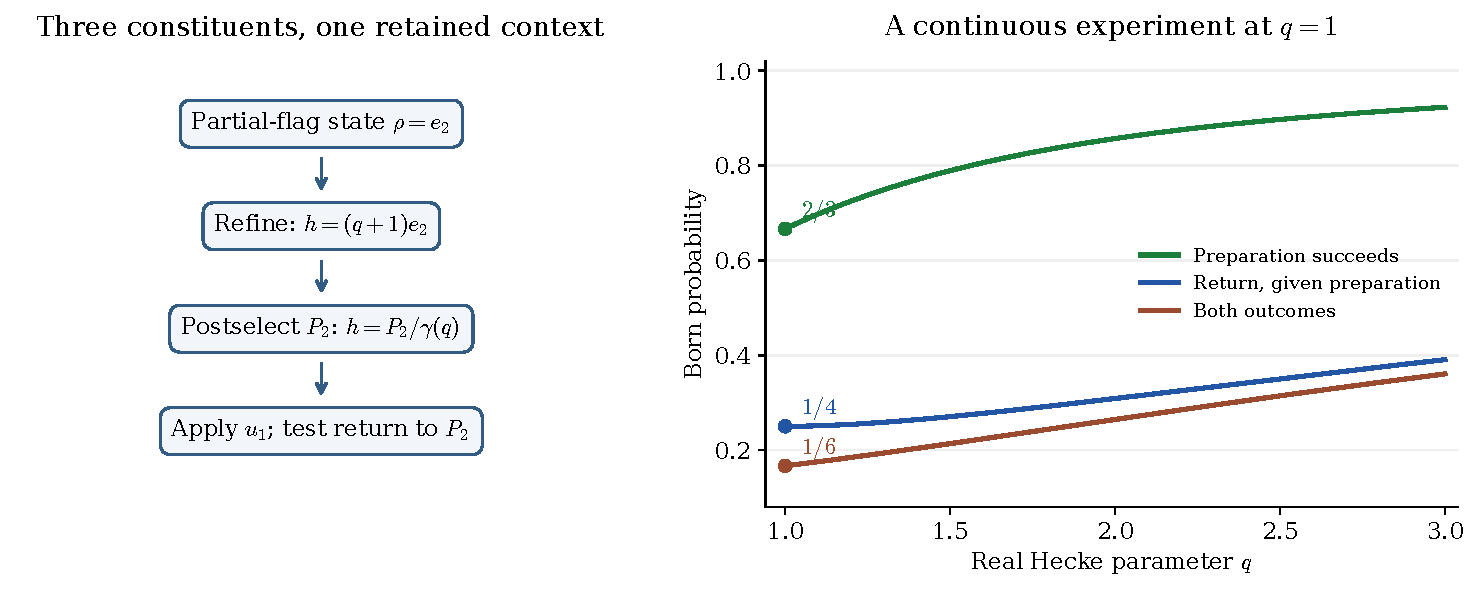
\includegraphics[width=\linewidth]{figures/f1-limit-protocol.pdf}
\caption{The three-constituent Lüders protocol.  Refinement is followed by
the specified backaction $K_s=P_2$, postselection succeeds with probability
$2/3$ at the endpoint, retained conjugation returns with conditional
probability $1/4$, and the joint endpoint probability is $1/6$.}
\label{fig:f1-limit-protocol}
\end{figure}
